In this section, we introduce the models and definitions used to describe ths
sybil attack, we use these in the remainder of the survey. Further, we give a
few impossibility results to illustrate the difficulty of the sybil attack

\begin{figure}
  \centering
  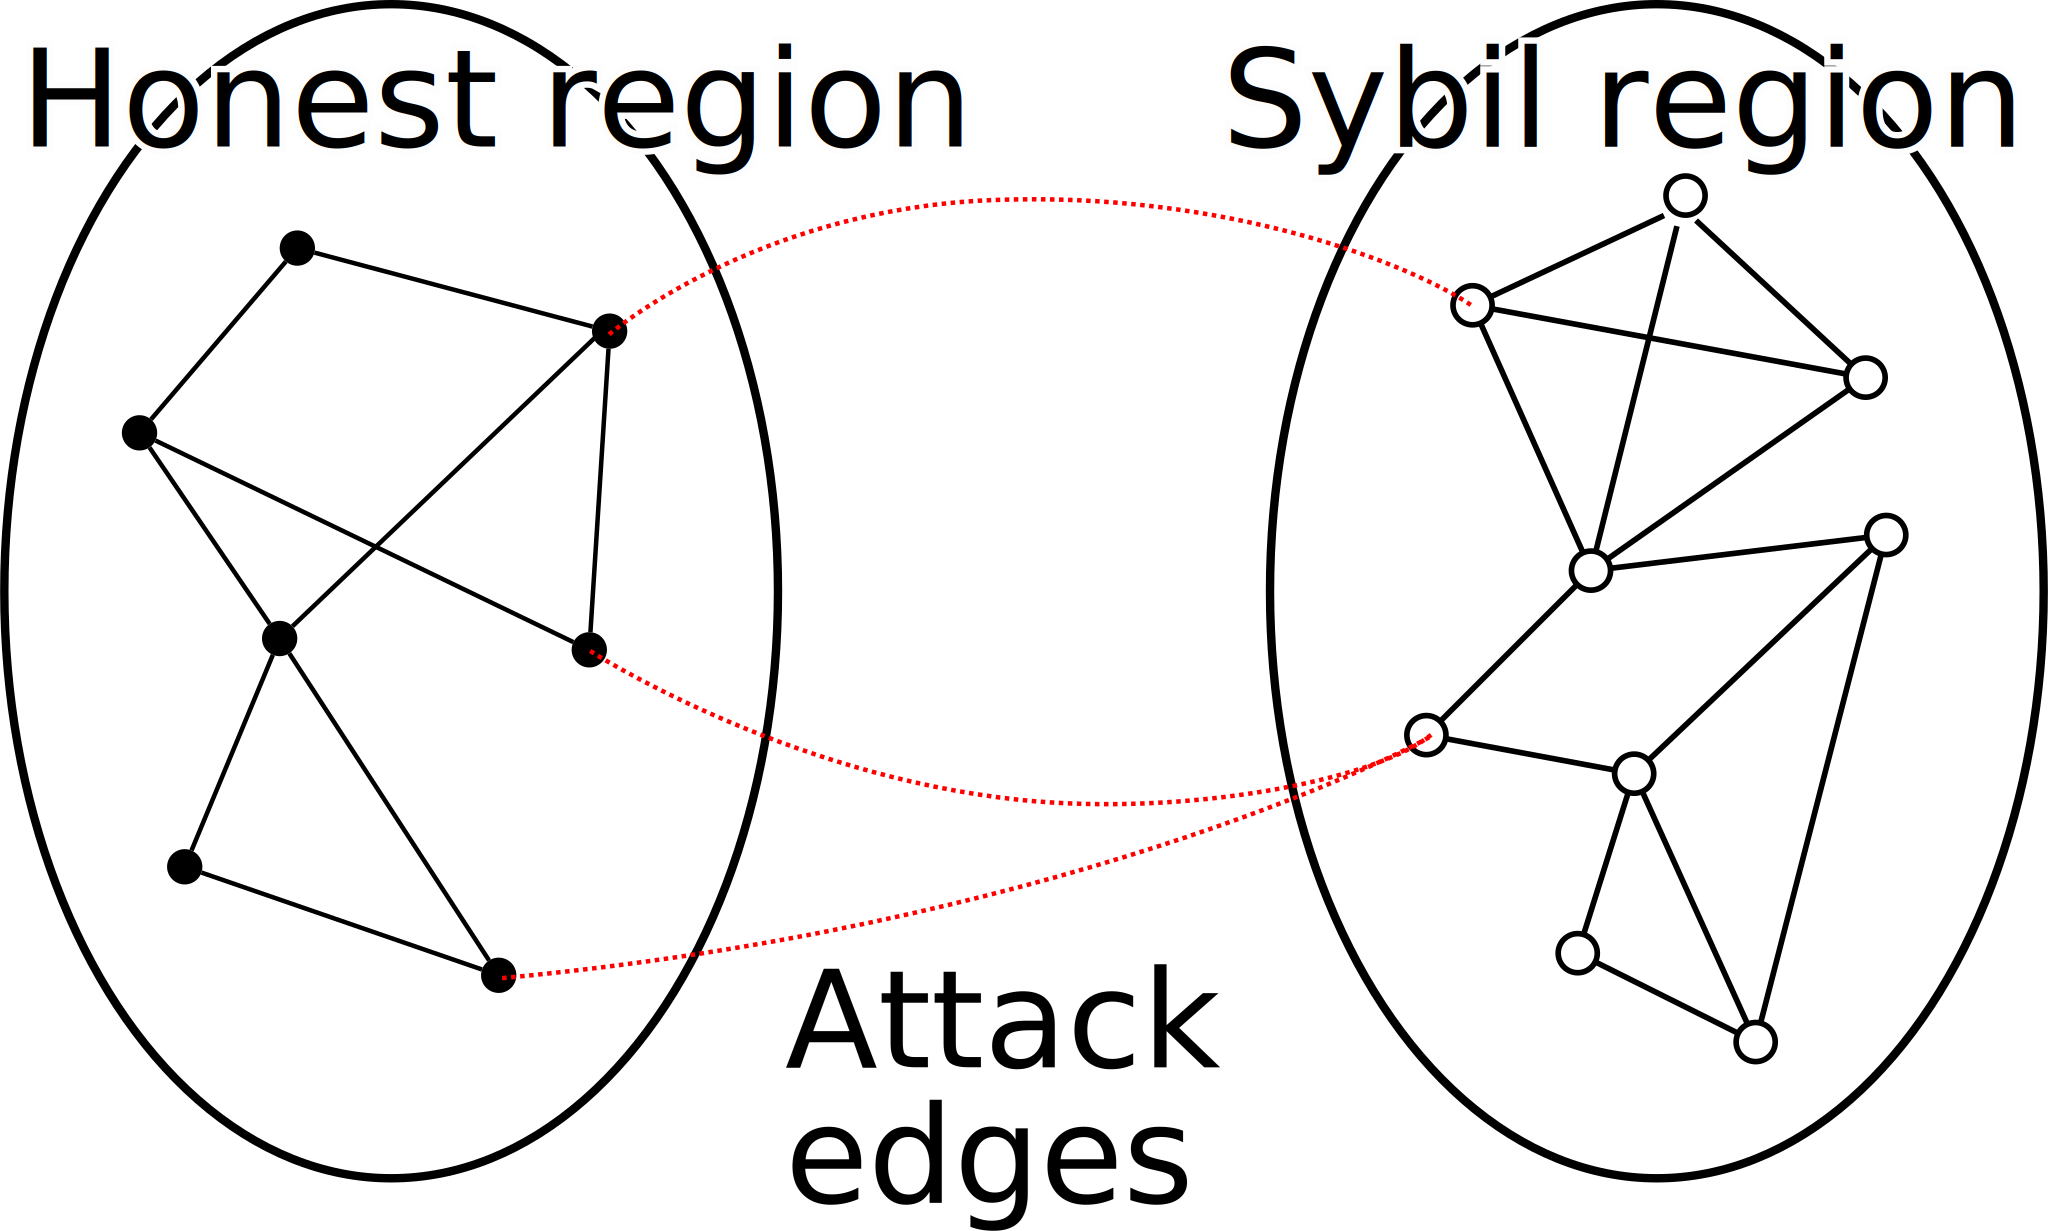
\includegraphics[width=\linewidth]{attack_edges}
  \caption{The model in many sybil defence mechanisms can be seen as a social
    graph that is partitioned into a sybil region and an honest region. The two
    regions are connected by \emph{attack edges}. Note that in general there may
    be multiple honest regions multiple sybil region. }
  \label{fig:attack-edge}
\end{figure}

\subsection{Definitions}
The sybil attack is coined by Douceur\cite{douceur2002sybil} in 2002 in the
context of P2P (peer-to-peer) systems. But people were well aware of it before
2002. For instance in 2001, Friedman and Resnick used the term ``cheap
pseudonyms'' to describe sybils~\cite{resnick2001social}. 

Douceur defined the sybil attack as forging multiple identities under the same
entity\cite{douceur2002sybil}. An entity can be for example a physical user of
the system and identities are how entities present themselves to the system.
Thus, a local entity has no direct knowledge of remote entities, only their
identities. The forged identities do not necessarily follow the protocol
specified by the underlying network, i.e. they assume the characteristics of
Byzantine fault\cite{lamport1982byzantine}. In this work, we use identity, node
and peer interchangeably.
% We use these terms in the remainder of the survey.

\subsection{Anonymous P2P Model}
The very first model on the sybil attack is proposed by Douceur. The system
under attack is modelled as a general distributed computing environment where
there is no constraint on the topology, every node has limited computational
resources and messages are guaranteed to be delivered~\cite{douceur2002sybil}.
Defending against the sybil attack is difficult under this model because nodes
can communicate with any other node without authentication or authorisation.
Only some techniques are able to defend against sybils under this model, we
describe them in \autoref{sec:network-flow}.

\subsection{Social Network Model}
The more common model, especially in the context of social networks, is shown in
\autoref{fig:attack-edge}. It is first introduced by the authors of
SybilGuard~\cite{yu2006sybilguard}. Nodes inside the left region are identities
created by honest entities, the edges connecting those nodes are real-world
trust relationships. The right region contains the sybils and they are connected
with fake relationships. The edges connecting the two regions are called
\emph{attack edges}. These can be created by tricking an honest user to befriend
a sybil, stealing an honest user's account and so on. We call the nodes in the
honest region that has one or more attack edges \emph{gullible nodes} or
\emph{victim nodes}. An important property of this model is that the number of
attack edges is not proportional to the number of sybils, but they are
proportional to the number of honest nodes. So if attackers create too many
sybils, then the graph will begin to have a quotient cut\footnote{Removing the
  attack edges will disconnect a large number of nodes from the social graph.}.
Many sybil defence mechanisms rely on the fact that attack edges are difficult
to create as we will describe in \autoref{sec:defences}.

\subsection{Impossibility Results}\label{sec:sybil-theory}
Under the anonymous P2P model, Douceur show that preventing the sybil attack is
in fact a lot more difficult because P2P systems often do not have a central,
trusted authority. In fact, the author prove that is it impossible to completely
prevent the sybil attack in a pure P2P environment.

Cheng and Friedman proved a very similar result in the context of reputation
systems~\cite{cheng2005sybilproof}. Reputation systems are commonly used in
e-commerce websites and the internet in general, where identities are rewarded
by their good behaviour or usefulness. Google's PageRank~\cite{page1999pagerank}
is an example of a reputation system, where many links to a website makes it
more reputable. It was formally proven that P2P reputation systems cannot be
made to prevent the sybil attack, it is only possible prevent it by using a
central, trusted authority.

% Cheng and Friedman proved an important result regarding the sybil attack in
% reputation systems\cite{cheng2005sybilproof}. Reputation systems are commonly
% used in MANET, e-commerce and the internet in general, where entities are
% rewarded by their good behaviour and penalised otherwise. Google's
% PageRank\cite{page1999pagerank} is an example of a reputation system, where a
% large number of links to a website makes it more reputable. Cheng and Friedman
% classified reputation systems into two categories,
% \begin{enumerate}
% \item symmetric reputation systems where the reputation score only depends on
%   the network topology, popular reputation mechanisms such as
%   PageRank\cite{page1999pagerank} and EigenTrust\cite{kamvar2003eigentrust} are
%   examples of symmetric reputation systems, and
%     \item asymmetric reputation systems where there some nodes are trusted and
%       reputation scores are propagated through the trusted nodes, most OSN are
%       examples of asymmetric reputation systems.
% \end{enumerate}
% The authors formally proved that symmetric reputation systems are vulnerable to
% the sybil attack. But in the asymmetric case, it is possible to construct a
% sybil-proof reputation system.

%%% Local Variables:
%%% mode: latex
%%% TeX-master: "main"
%%% End:
